\documentclass{beamer}

\usepackage{beamerthemebars}
\usepackage{amsmath, amssymb}
\usepackage[utf8]{inputenc}
\usepackage[ngerman]{babel}
\usepackage{url}
\usepackage{algorithm2e}
\usepackage{graphicx}
\usepackage{wrapfig}
\usepackage[font={small}]{caption}

\setbeamertemplate{footline}[frame number]
\setbeamertemplate{caption}{\raggedright\insertcaption\par}

\begin{document}

\date{28. August 2019}
\title{Softwarepraktikum "Parallele Numerik"}
\subtitle{Abschlussvortrag}
\author{Rebecca Seelos, Alexander Lüngen, Joshua}

\frame{
  \titlepage
}



% TODO: 
% - Code für Rechenvorschrift (MATH)
% - Grafik für Rechenvorschrift - Neighbor problem
% - 
\section{Problemstellung}%Joshua
\frame{
    \frametitle{Gegeben}
    \begin{itemize}
        \item Maße der Hertplatte
        \item Anfangstemperatur
        \item Randtemperatur
        \item Wärmezufuhr
    \end{itemize}
}

\frame{
    \frametitle{Gesucht}
        \begin{itemize}
        \item Wärmeverteilung
        \item Wärmeentwicklung über Zeit
        \item Zeit bis zu einer bestimmten Temperatur
    \end{itemize}
}

\frame{
    \frametitle{Teilaufgaben}
        Finden einer geeigneten ...
        \begin{itemize}
        \item ... Methodik zum Lösen von Gleichungen
        \item ... Parallelisierungsmethode
        \item ... Programmiersprache zur Implementierung
    \end{itemize}
}

\section{Parallelisierung}
\frame{
	\frametitle{Gauß-Seidel Verfahren - Motivation}
 Im Rahmen der Finiten Elemente Methode müssen häufig Gleichungen gelöst werden:\\
\rightarrow Welche Gleichungen?\\
\rightarrow Gauß-Seidel-Verfahren\\
	 Iteratives Verfahren um lineare Gleichungen näherungsweise zu lösen\\
}
\frame{
    \frametitle{Gauß-Seidel Verfahren - Anwendung}
    
    \begin{description}
        \item[1. Gegeben das Gleichungssystem:] \hfill
            $ a_{11} * x_1 + a_{12} * x_3 + ... + a_{1n} * x_n = b_1 $ \\
	        $ \qquad  \vdots \qquad \qquad \qqaud \vdots \qquad \qqaud \qquad \vdots $ \\
	        $ a_{n1} * x_1 + \qquad ...  \qquad + a_{nn} * x_n = b_n $ \\
        
        \item[2. Wähle Startvektor:] \hfill \\ 
            $x^0 \in \mathbb{R}^n$
        
        \item[3. Iteriere über Vektoreinträge einen Schritt mit der Vorschrift:] \hfill \\
            $\forall k = 0,1,\dots; \quad \forall j = 1,..,n : \\ $
            $\quad x_j^{k+1} = \frac{1}{a_{j,j}} \left( b_j - \sum\limits_{i=1}^{j-1} a_{j,i}x_{i}^{k+1} - \sum\limits_{i=j+1}^{n} a_{j,i}x_{i}^k \right) $
        
    \end{description}
}

\frame{
	\frametitle{Parallelisierungsmethoden}
	Parallelisierung des Gauss-Seidel-Verfahrens
    \begin{enumerate}
        \item Wavefront
        \item Diamondtiling
        \item Jacobi-Iteration
    \end{enumerate}
}

\frame{
    \frametitle{Parallelisierungsmethoden - Wavefront}
    
    Problem:
    - unregelmäßiger Parallelisierungsgrad
    Optimierungsmöglichkeit:
    - Freigabe von zuvor berechneten elementen für den nächsten Schritt
}

\frame{
	\frametitle{Parallelisierungsmethoden - Diamondtiling}
    	\begin{figure}
	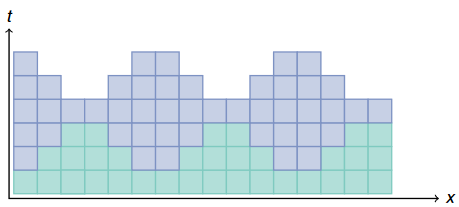
\includegraphics[width=\linewidth]{figs/Diamondtiling.png}
	\caption{Quelle: Vorlesung  \dq Software Engineering für moderne parallele Plattformen\dq, Foliensatz  \dq2.Entwurf\dq}
\end{figure}
}

% 
\frame {
    \frametitle{Parallelisierungsmethoden - Jacobi-Iteration}
    Verändern der Rechenvorschrift von Gauß-Seidel-Verfahren
    
    Neue Rechenvorschrift:
    
    $ x^{k+1} = \frac{1}{a_{i,i} \left(   \right)} $
    
    % TODO Figur zum Schachbrettmuster
    
    \begin{description}
        \item[Datenabhängigkeit nur im gleichen Zeitschritt]
        \item[Wähle optimal bzgl. Speicher vs. Parallelisierungsgrad]
    \end{description}
    
}
% ENDE ############ kram von Alex

% ########## KRAM von REBECCA
\section{OpenMP und CUDA}
\frame{
	\frametitle{OpenMP}
	Beispiele aus dem Praktikum: Numerische Berechnung von $\pi$, Mandelbrot, Gauss-Seidel\\
	
	
	Die Vorteile sind: 
    \begin{itemize}
    	\item einfach in existierenden Code zu integrieren mit entsprechenden '\#pragma'
    	\item mit dem gcc compiler zu nutzen
    \end{itemize}
}
\frame{
	\frametitle{OpenMP Nachteile}
	
	\begin{itemize}
	    \item Korrekte Anwendung wichtig
	    \item verleitet eventuell dazu Dinge zu einfach zu sehen
	\end{itemize}
}

\frame{
    \frametitle{Beispiel: Gauß-Seidel}
    	\begin{tabular}{|l|l|l|l|r|}
		\hline
		Implementierung & l,h &T(1) & T(n)(parallel) & S(n)\\
		\hline
		OMP naiv & l=5, h=1/32 & 1.42 & 1.154 & 1.231 \\
		\hline
		OMP naiv & l=6; h=1/64 & 37.216s & 26.884s & 1.384 \\
		\hline
		OMP Jacobi & l=5, h=1/3 & - & 1.475s & 0.963 \\
		\hline
		OMP Jacobi & l=6, h=1/64 & - & 6.394s & 5.82 \\
		\hline 
	\end{tabular}
}

\frame{
	\frametitle{CUDA}
	Vorteile:
	\begin{itemize}
	    \item Nutzung der GPU (von NVIDIA)
	    \item gut bei hoher Datenparallelität
	\end{itemize}
	
	Nachteile:
	\begin{itemize}
	    \item bedarf Einarbeitung
	    \item nvcc compiler, verschiedene Versionen von Grafikkarten, manchmal nicht kompatibel - angewiesen auf Hardware 
	    \item overhead
	\end{itemize}
}
\frame{
	\frametitle{Beispiel: Vector inkrementieren}
	Zeit mit OpenMP auf CPU: 488.875 ms
	\begin{center}
	    \begin{tabular}{l|l|l|}
		\cline{2-3}
		& \multicolumn{2}{c|}{Speedup} \\ \hline
		\multicolumn{1}{|l|}{blocksize} & Time      & N = 10ˆ8     \\ \hline
		\multicolumn{1}{|l|}{4}         & 141.23ms  & 3.49         \\ \hline
		\multicolumn{1}{|l|}{32}        & 18.020ms  & 27.74        \\ \hline
	\end{tabular}
	\end{center}
}

\frame{
    \frametitle{Beispiel: Gauß-Seidel}
    	\begin{tabular}{|l|l|l|l|r|}
		\hline
		Implementierung & l,h & T(1) & T(n) & S(n)\\
		\hline
		OMP naiv & l=5, h=1/32 & 1.42s & 1.154s & 1.231 \\
		\hline
		OMP naiv & l=6; h=1/64 & 37.216s & 26.884s & 1.384 \\
		\hline
		OMP Jacobi & l=5, h=1/3 & - & 1.475s & 0.963 \\
		\hline
		OMP Jacobi & l=6, h=1/64 & - & 6.394s & 5.82 \\
		\hline 
		CUDA Jacobi & l=5, h=1/32 & - & 1.055s & 1.346 \\
		\hline
		CUDA Jacobi & l=6, h=1/64 & - & 1.318s & 28.237 \\
		\hline
	\end{tabular}
}
% ############## Ab hier Part von Joshua ##############
\section{Partielle Differentialgleichungen}


\frame{%Projekt1 Aufgabe 5
	\frametitle{Finite-Differenzen-Methode}
		\begin{figure}
	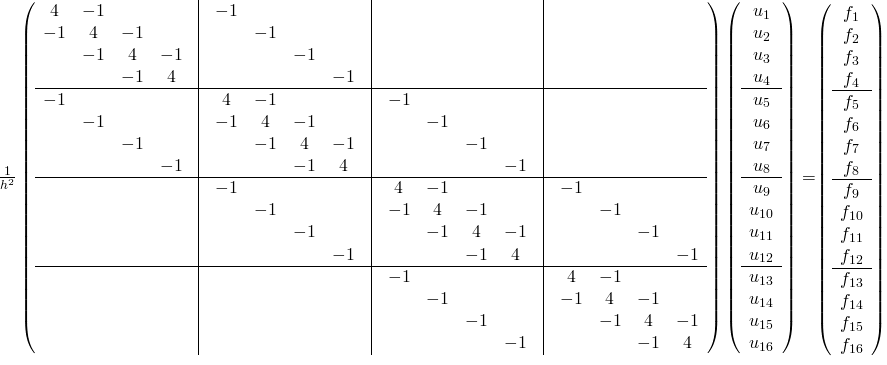
\includegraphics[width=\linewidth]{figs/matrix.png}
\end{figure}
}



\frame{
	\frametitle{Krylow-Unterraumverfahren \& GMRES}%Joshua
		\begin{itemize}
	\item iterative Verfahren zum Lösen großer, dünnbesetzter Gleichungssysteme
	\item GMRES = Generalized minimal residual method
	\item Begrenzte Anzahl der Schritte bis zum Konvergenz
	\item Residuum abschätzen um Operationen zu sparen
	\end{itemize}
}
\frame{
	\frametitle{Vergleich GMRES - Gauss-Seidel-Verfahren}%Joshua
	\begin{table}
	\centering
\begin{tabular}{|l|l|r|r|}
		\hline
		- & Gauss-Seidel(s) & GMRES(s) & Speedup\\
		\hline
		l=5; h=1/32 &0.488 & 0.025  &  19.52 \\
		\hline
		l=6; h=1/64 &0.960 & 0.135  &  7.11 \\
		\hline
		l=7; h=1/128 &8.856 & 1.300 & 6.812 \\
		\hline
	\end{tabular}
\end{table}
}

\frame{
	\frametitle{LU-Zerlegung}%Joshua
	\begin{itemize}
	    \item Weitere Verbesserungen durch Vorkonditionierung
	    \item $A = (L*U)^{-1}$
	    \item GMRES konvergiert schneller
	\end{itemize}
}
\section{Simulation}%Joshua
\frame{
	\frametitle{Rand- und Anfangsbedingungen}
	\begin{itemize}
\item $- \triangle u(x,y,t_{n}) = \frac{f(x,y)-u'(x,y,t_{n})}{a}   ,$   $  (x,y) \in \Omega = (0,1)^2  ,$   $  n \in N\backslash0;$\\

\item $u(x,y,t_{n}) = 20,$   $(x,y) \in \Gamma ,$   $ n \in N;$\\
\item $u(x,y,t_{0}) = 20,$   $ (x,y) \in \Omega ; $ \\
\item f(x,y) ist stetig,   $ (x,y) \in \Omega .$ \\
\end{itemize}
}
\frame{
\frametitle{Zeitschritt}
\begin{itemize}
\item $u'(t_{n})  = f + a * \triangle u(t_{n})$\\
mit $\triangle u(t_{n}) =  \frac{4*u_{i,j}(t_{n})-u_{i-1,j}(t_{n})-u_{i+1,j}(t_{n})-u_{i,j-1}(t_{n})-u_{i,j+1}(t_{n})}{h_{s}^{2}}$\\
\item$u(t_{n+1})  =u(t_{n}) + h_{t} * u'(t_{n})$\\
\item$A* u(t_{n}) = \frac{h_{s}^{2}}{a} * ( f-\frac{ u(t_{n}) -  u(t_{n-1})}{h_{t}}) $\\
\end{itemize}
}
\frame{
	\frametitle{Implementierung}
	\begin{itemize}
	\item OpenMp
	\item Vorkonditioniert
	\item GMRES (mit Residuumschätzung)
	\end{itemize}
}
\frame{
	\frametitle{Ergebnisse}
	\begin{figure}
	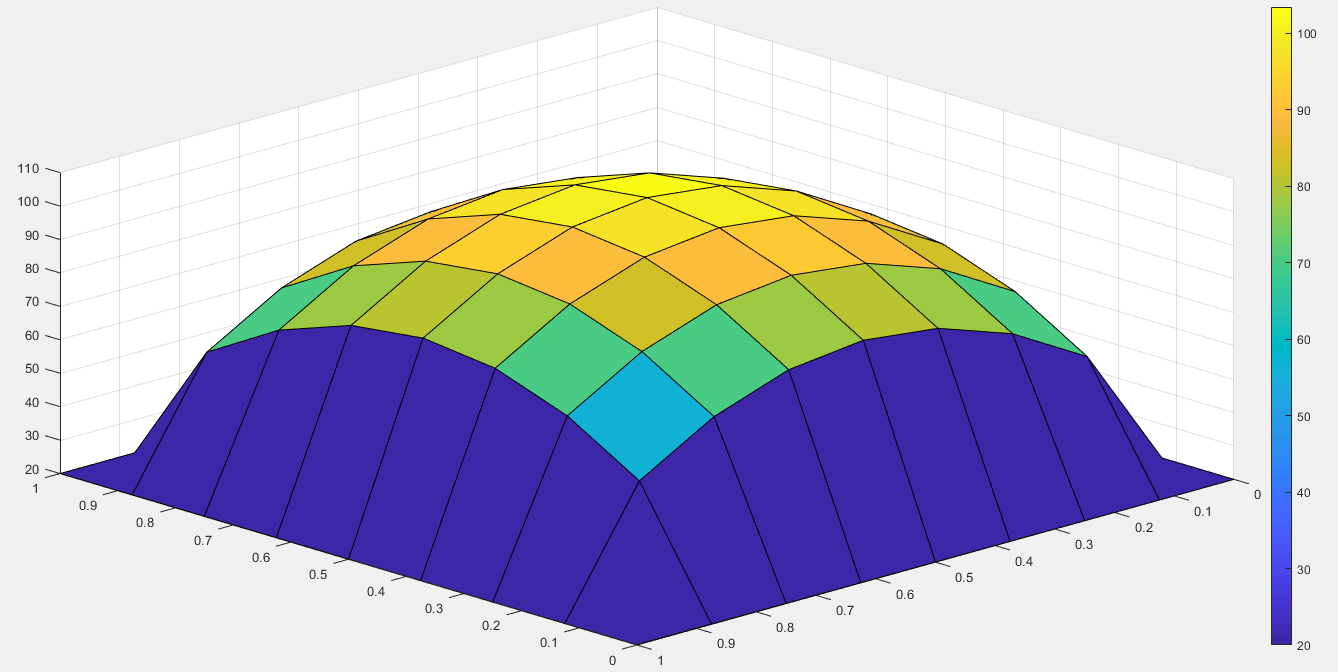
\includegraphics[width=\linewidth]{figs/P2A5T60.png}
\end{figure}
}
\frame{
	\frametitle{Ausblick}
	\begin{itemize}
	\item Simulation weiter verschnellern (CUDA - GPU)
	\item Beliebige Hertplattenformen zulassen (zB. Kreis)
	\item Mit der Simulation optimieren (Abbruchbedingung anpassen?)
	\end{itemize}
}

\frame{
	\frametitle{Fragen?}
	Danke für Ihre Aufmerksamkeit!
}
\end{document}



%%% Local Variables: 
%%% mode: latex
%%% TeX-master: t
%%% End: 
